\documentclass[conference]{IEEEtran}
\IEEEoverridecommandlockouts
% The preceding line is only needed to identify funding in the first footnote. If that is unneeded, please comment it out.
\usepackage{cite}
\usepackage{amsmath,amssymb,amsfonts}
\usepackage{algorithmic}
\usepackage{graphicx}
\usepackage{textcomp}
\usepackage{xcolor}
\def\BibTeX{{\rm B\kern-.05em{\sc i\kern-.025em b}\kern-.08em
    T\kern-.1667em\lower.7ex\hbox{E}\kern-.125emX}}
\begin{document}

\title{Simple Action Model: Enabling LLM to Sequential Function Calling Tool Chain\\
}

\author{
% \IEEEauthorblockN{\textsuperscript{} Angel Rose Benny} 
% \IEEEauthorblockA{\textit{ Department of AI\&DS} \\
% \textit{SJCET Palai}\\
% Kottayam, Kerala \\
% bennyangelrose@gmail.com
% }
% \\
% \IEEEauthorblockN{Jowin Joseph Raju} 
% \IEEEauthorblockA{\textit{ Department of AI\&DS} \\
% \textit{SJCET Palai}\\
% Kottayam, Kerala \\
% jowincraju@gmail.com}

% \and
\IEEEauthorblockN{Rajat Sandeep Sen}
\IEEEauthorblockA{\textit{ Department of AI\&DS} \\
\textit{SJCET Palai}\\
Kottayam, Kerala \\
rajatsandeepsen2025@ai.sjcetpalai.ac.in}

\\
\IEEEauthorblockN{Neena Joseph}
\IEEEauthorblockA{\textit{ Department of AI\&DS} \\
\textit{SJCET Palai}\\
Kottayam, Kerala \\
neenajoseph@sjcetpalai.ac.in}




% \and

% \IEEEauthorblockN{Jeevan George}
% \IEEEauthorblockA{\textit{ Department of AI\&DS} \\
% \textit{SJCET Palai}\\
% Kottayam, Kerala \\
% jeevang1975@gmail.com}



}

\maketitle

\begin{abstract}
 Today LLMs are everywhere, it is making human internet life a lot easier than ever.
Everyday new sophisticated models are releasing. But these models are not good enough to become
the personal assistant like the Jarvis from Sci-fi movie IronMan. This paper proposes
a way to enable any LLM to execute complex requirements in real world applications. By
leveraging state-of-the-art Large Language models, we can create a simple action model that can 
understand environment around them. Eventually these models can help or assist humans in real time applications.
The Sequential Function Calling Tool Chain System
aims to bridge the gap between human language understandings and computer programming.
\end{abstract}

\begin{IEEEkeywords}
Large language model, Action model, OpenAPI format and Function Calling Tools
\end{IEEEkeywords}

\section{Introduction}
Now on a world without AI is impossible to imagine. New models will comes everyday, and new architecture will improve its performance. Multi Modality or Mixture of Models are not enough to become the personal assistant. Graph based models takes up lot of computation in the case of complex function calling. Simple Question, "what if the one good model with one request is enough to execute multiple functions sequentially?".

The integration of openAPI schema with LLM can make a decent action model that can understand the API specs of that specific applications. The large language model will take prompts and decides what to do. From programming side, we'll parse the information and execute. Simple action model is done. 

By implementing a custom JSON parser alongside with an OpenAPI schema type system it is possible to utilize one model as main decision making inside an application. This technology works faster compared to other solutions, but requires much more intelligent language model.

This helps to provide stable and intelligent AI assistant in any applications uphold the integrity and standards API formats. This research paper also leads to the exploration of Multiple and Sequential Function calling tool chain that utilizes State-of-the-Art Language model to enhance the security, time efficiency,flexibility for building AI applications. 

Purpose of this paper is to explore and improve existing solutions of Function calling tools available in open source software community. This paper also aims to provide a new approach to prompting the LLMs without fine tuning.

\section{Literature Survey}
These literature reviews provides knowledge about the existing researches done by various scholars and open source developers. 
% [1] Tong Liu ,AI Proctoring for offline examinations with 2-Longitudinal-Stream Convolutional Neural Networks 10 December 2022, has used two  Convolution Neural Networks to implement the 
% the AIPS (AI Proctoring System).The first Convolution Neural Network is used to detect the human face that received in the frame.The second convolution network is used to detect the action of humans is the frame detected by frame 1.This is implemented using the Tensorflow and Keras.Disadvantage that lead to this paper is the detection of malpractise is limited.AIPS will declare an examine is cheating if he/she lifts his/her face from the answer sheet.If an examine cheats during exam with head down position then it will not be detected.
% [2] Musa Dima Genemo,Suspicious activity recognition for monitoring cheating in exams 24 February 2022, They had utilised the L4-Branched ActionNets(L4BANs).
% The two distinct datasets used by them are CUI ExamDataset and CIFAR-100 DataSet those are most well known data in the field of image classification in exam proctoring systems.
% [3] Categorizing the Student's Actvities for  Automated Exam Proctoring using Proposed Deep L2-Grafnet CNN Network and Feature Selection Approach by Muhammad Sharif assisted by Amjad Rehman.In this research paper the had used Deep Learning Approach for the analysis of categorization of student activities during exam.A new deep CNN Architecture  with 46 layers is proposed which contains the characteristics of deep AlexNet and Squeezenet.The proposed model is first coverted to a pretrained model by performing its traing with Softmax Classifier with the CIFAR-`100 dataset.The optimized features are passed to different variants of SVM and KNN Classifier.Thew output is obtained with a huge accuracy of 93.88 percentage using fine knn classifier.
%   [4] Joseph Redmon,Santosh Divvala ,Ross Girshick,Ali Farhadi You Only Look Once:Unified Real-Time Object Detection 9 May 2016 ,It uses Convolution Neural Networks.Its unified Architecture enables efficient detection of objects across different classes.YOLO provides high accuracy and real time performance. [5] Rhitvik Pasricha ,Prathamesh  Churi ,A Systematic Review on AI-Bsed proctoring Systems:Past, Present,Future  September 2021.AIPS are increasingly popular for maintaining exam integrity .Security corncerns with AIPS are also increasing and they are impacting acceptance and exam results. OPS (Online Proctoring Systems) focuses on webcam recording and browser lockdown.Technical factors like network stability and human psychology affect proctoring effectiveness. 
\section{Methodology}
The approach of Sequential Function calling tool is using the popular and newest OpenAPI schema 3.0. By fetching the schema json from the backend url is converted to type parser like Zod (npm) at build time. The prompt captured from the user is fed to LLM with proper type annotation of OpenAPI schema. Any popular open source model can be used to understand and extract object/json data from users prompts. The extracted data are then loaded into a custom JSON parser that supports extra keywords from standard JSON format. The parser moves the data to OpenAPI clients libraries like OpenAPI-Fetch (npm) which fetch result from the backend. The result is then passed to the next function in the chain. The process is repeated until the end of the chain. But LLM is used once just to write "what to do in this environment" according to users prompts and type definition.

\subsection{Schema Preparation}\label{AA}
The preparation of the schema at build time utilizes popular libraries like OpenAPI-TS (npm) and OpenAPI-Zod (npm). It'll generate types schema for using in few-shot learning of LLM and zod schema for parsing the input and return data to and from LLM. Feeding the LLM with raw OpenAPI schema is waste of tokens and context window, that's why it is a crucial step to create simpler version of schema. This process involves collecting openAPI schema JSON (by fetching from application backend server), parsing and preprocessing, and then structuring it in a way that is useful for teaching the language model. 

The recorded schema were obtained from backend frameworks that supports swagger-ui or other libraries that generates OpenAPI. Simplified parser schema and type are written to coding file (here typescript programming language is used) and saved into a folder. Later these obtained schema were resized to smaller chunks if schema is larger that models context window. Graph based structure is used to label and store nodes. This graph data structure will help to query through large schema faster in runtime. 

\begin{figure}[htbp]
    \centering
    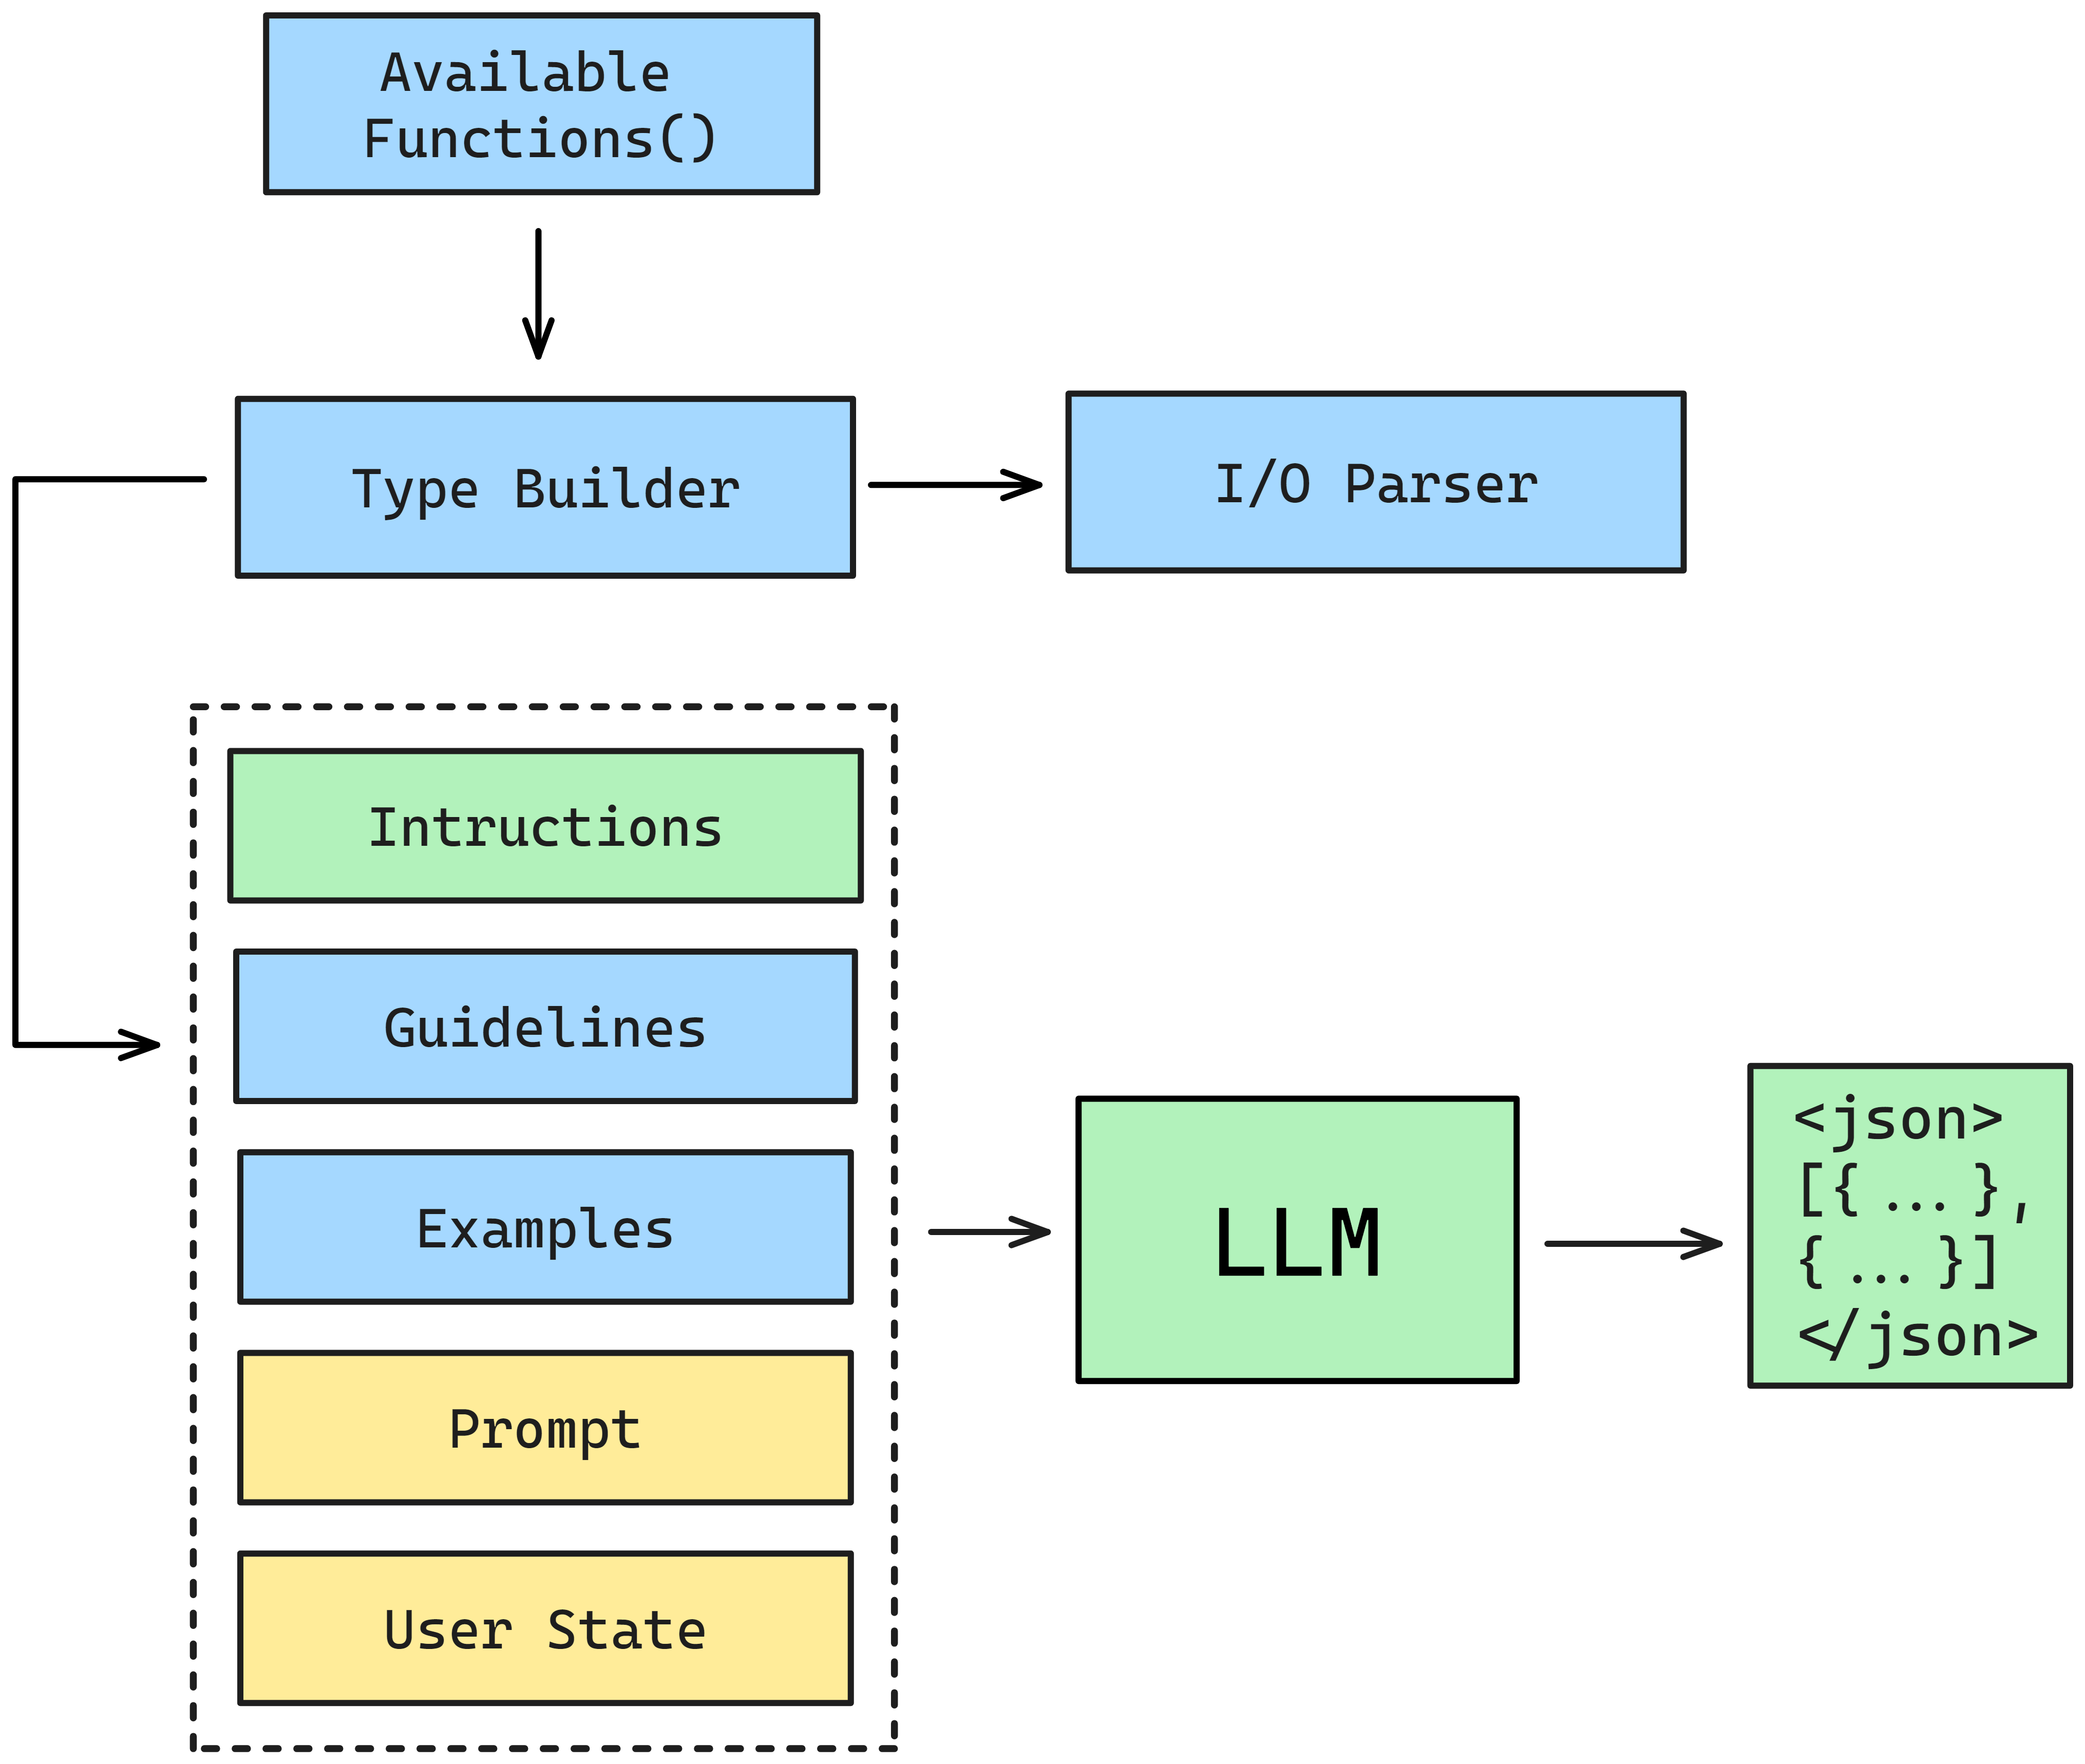
\includegraphics[width=0.5\textwidth]{images/without-finetuning.png}  
    \caption{Block Diagram for Normal In-context Learning}
    \label{fig}
\end{figure}

\subsection{Prompt Preparation}
Alway the LLM is instructed to return response in <JSON> tags, making the data easier to extract from string. Also available functions list (or schema from OpenAPI) is converted to easy type definitions, which makes easier to understand by the LLMs. 

But normally open source LLMs are stupid without examples. They are trained on general knowledge, that why its important for few shot in-context learning to make it understand the environment.

Also fine tuning approach is also great if type definition and instructions is larger than context window of the LLM using. Teach the Model with entire OpenAPI schema and examples before deploying to production give better result in response and saves lot of tokens while prompting each time. 

\begin{figure}[htbp]
\centering
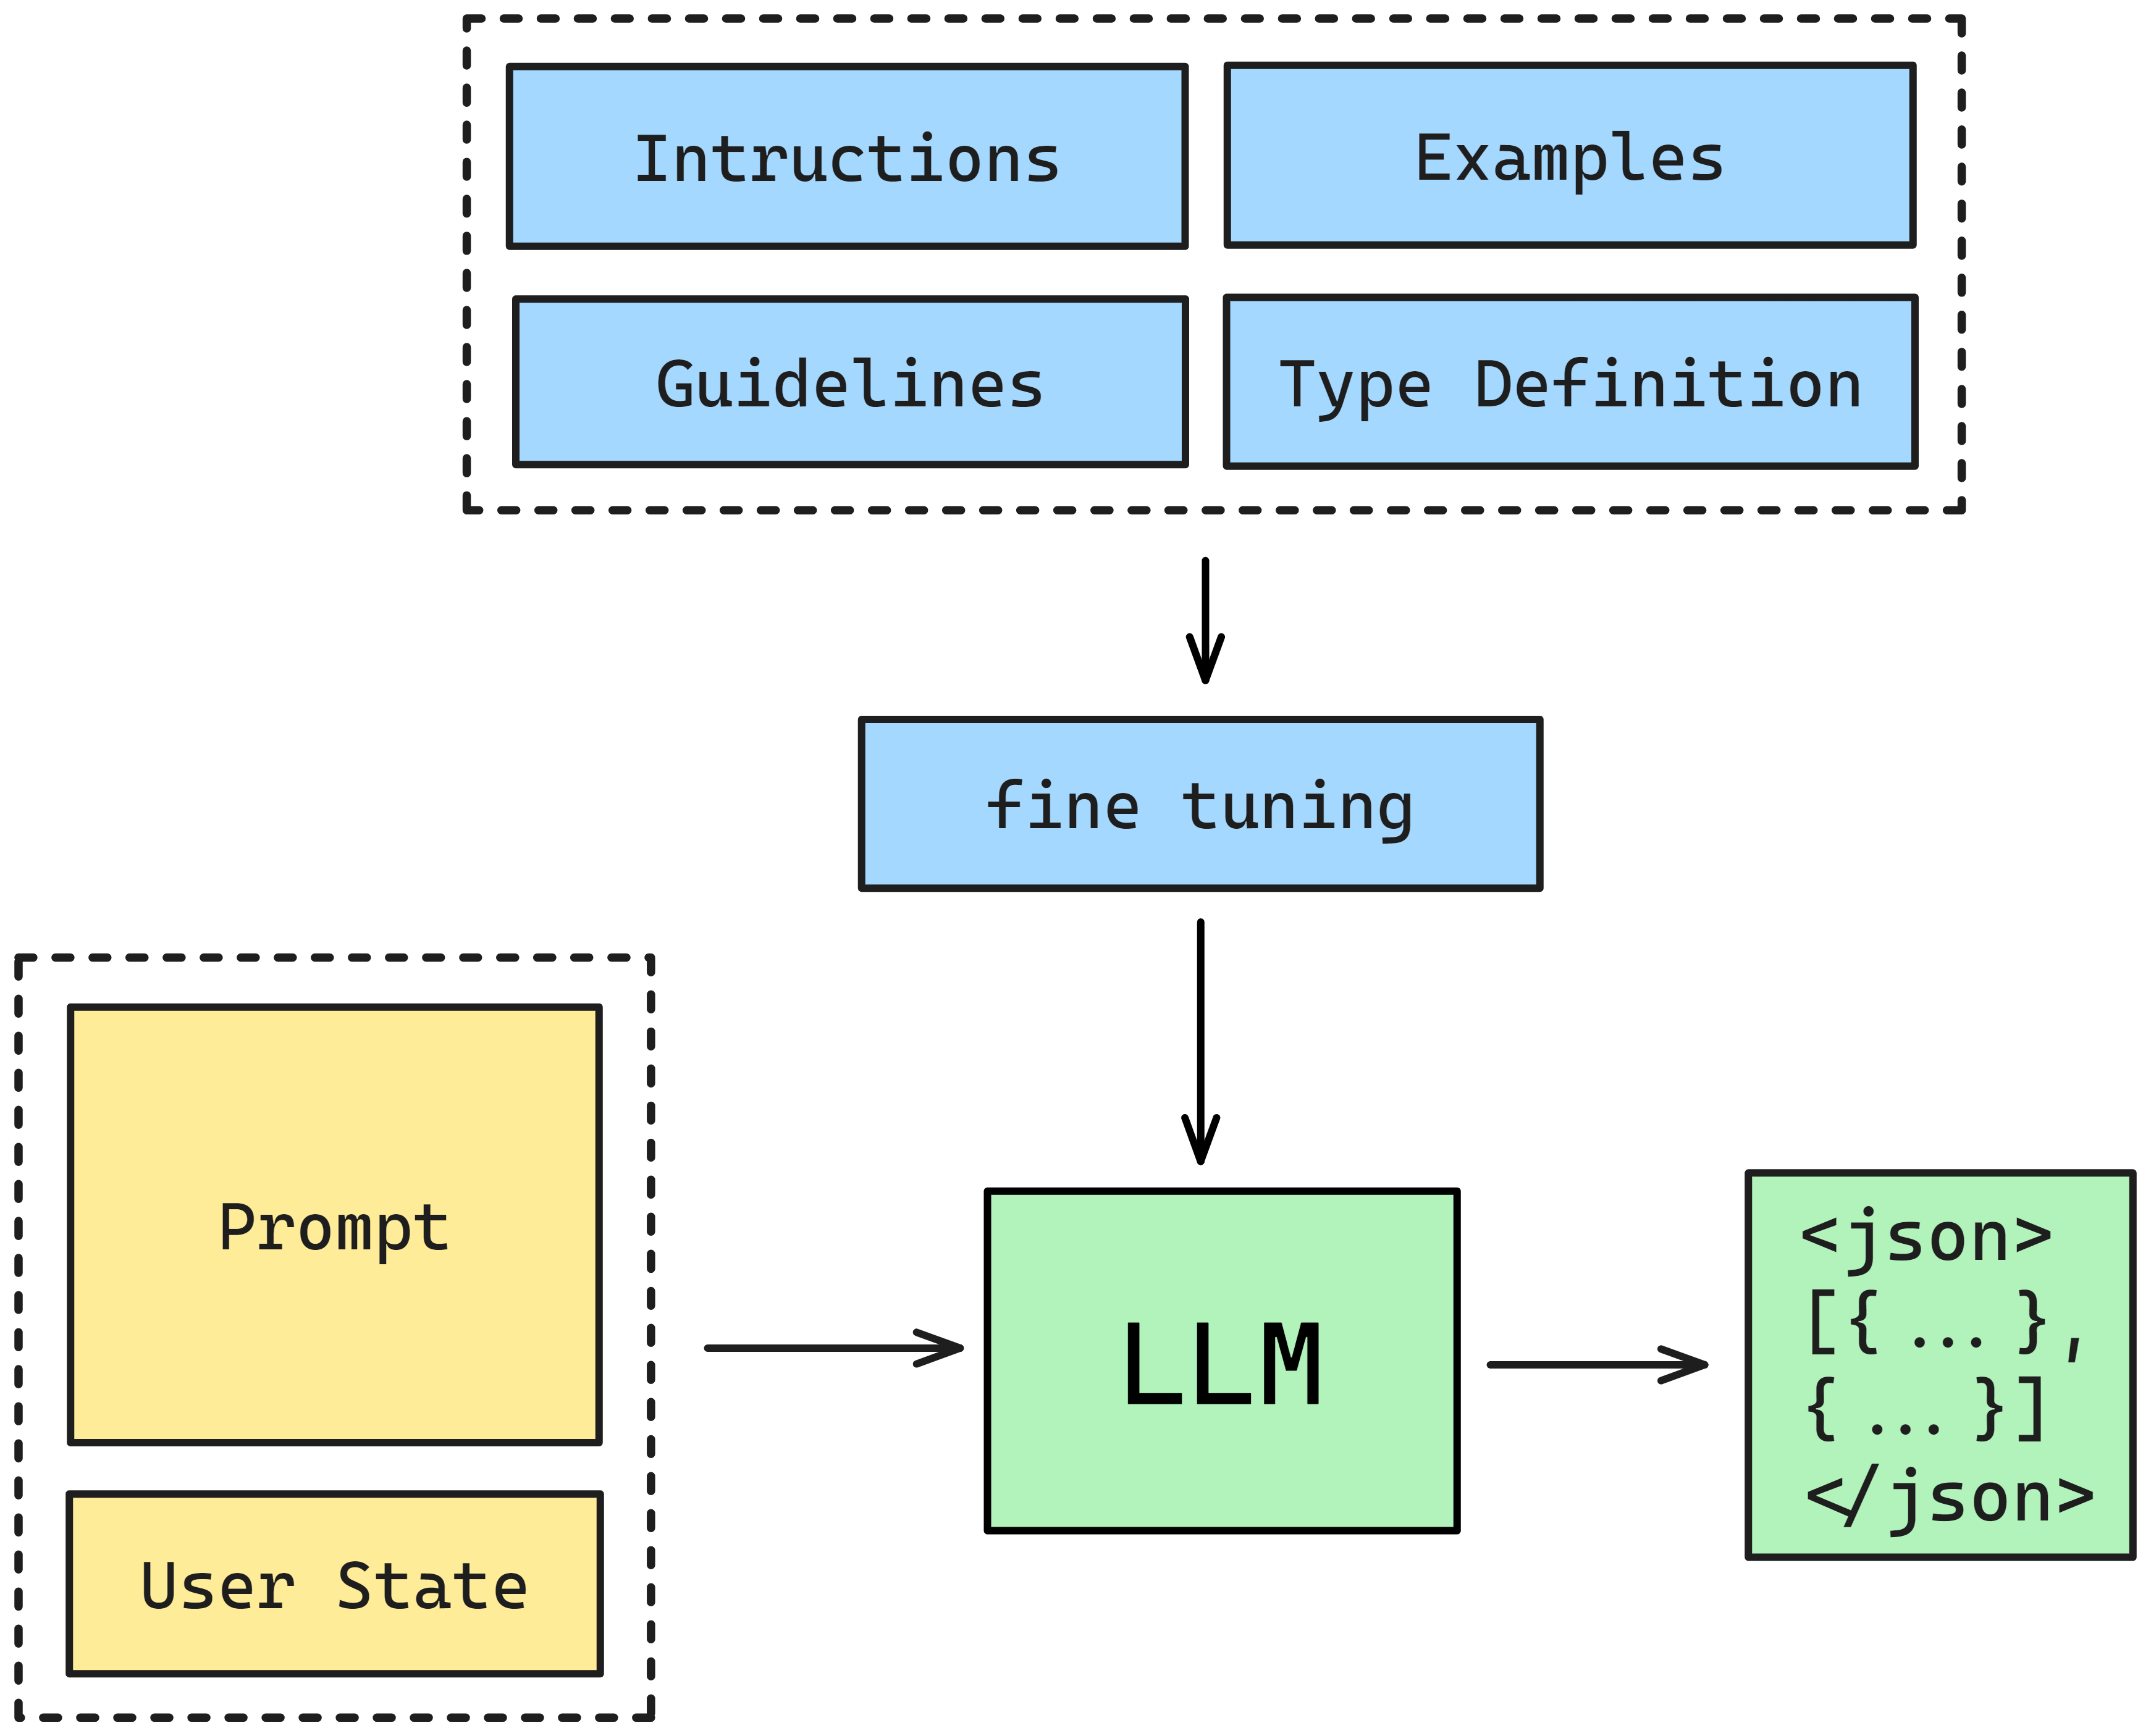
\includegraphics[width=0.5\textwidth]{images/fine-tuned.png}  
\caption{Block Diagram for Fine tuned learning}
\label{fig}
\end{figure}

\subsection{Server Architecture}
Initially developer specifies the backend URL and OpenAPI schema URL in the configuration file. The CLI fetches the schema from the backend applications and preparation the schema at build time. The server is an standalone backend that listens to end users prompts. Server takes user prompt, type definition of OpenAPI schema and sends to LLM. The developer also need to mentions the provider and model in configuration file. Then the LLM return with some JSON data wrapped with <JSON> tag. The data shows "what to run", "where to fetch" and "what are the parameter and request body". The server then parses the JSON data and sends to the Action engine. The engine take care of function calling and chaining. Finally the result is sent back to user in JSON format (or stream the UI if server is built with meta-frameworks like Next.js or Nuxt.js).

\begin{figure}[htbp]
    \centering
    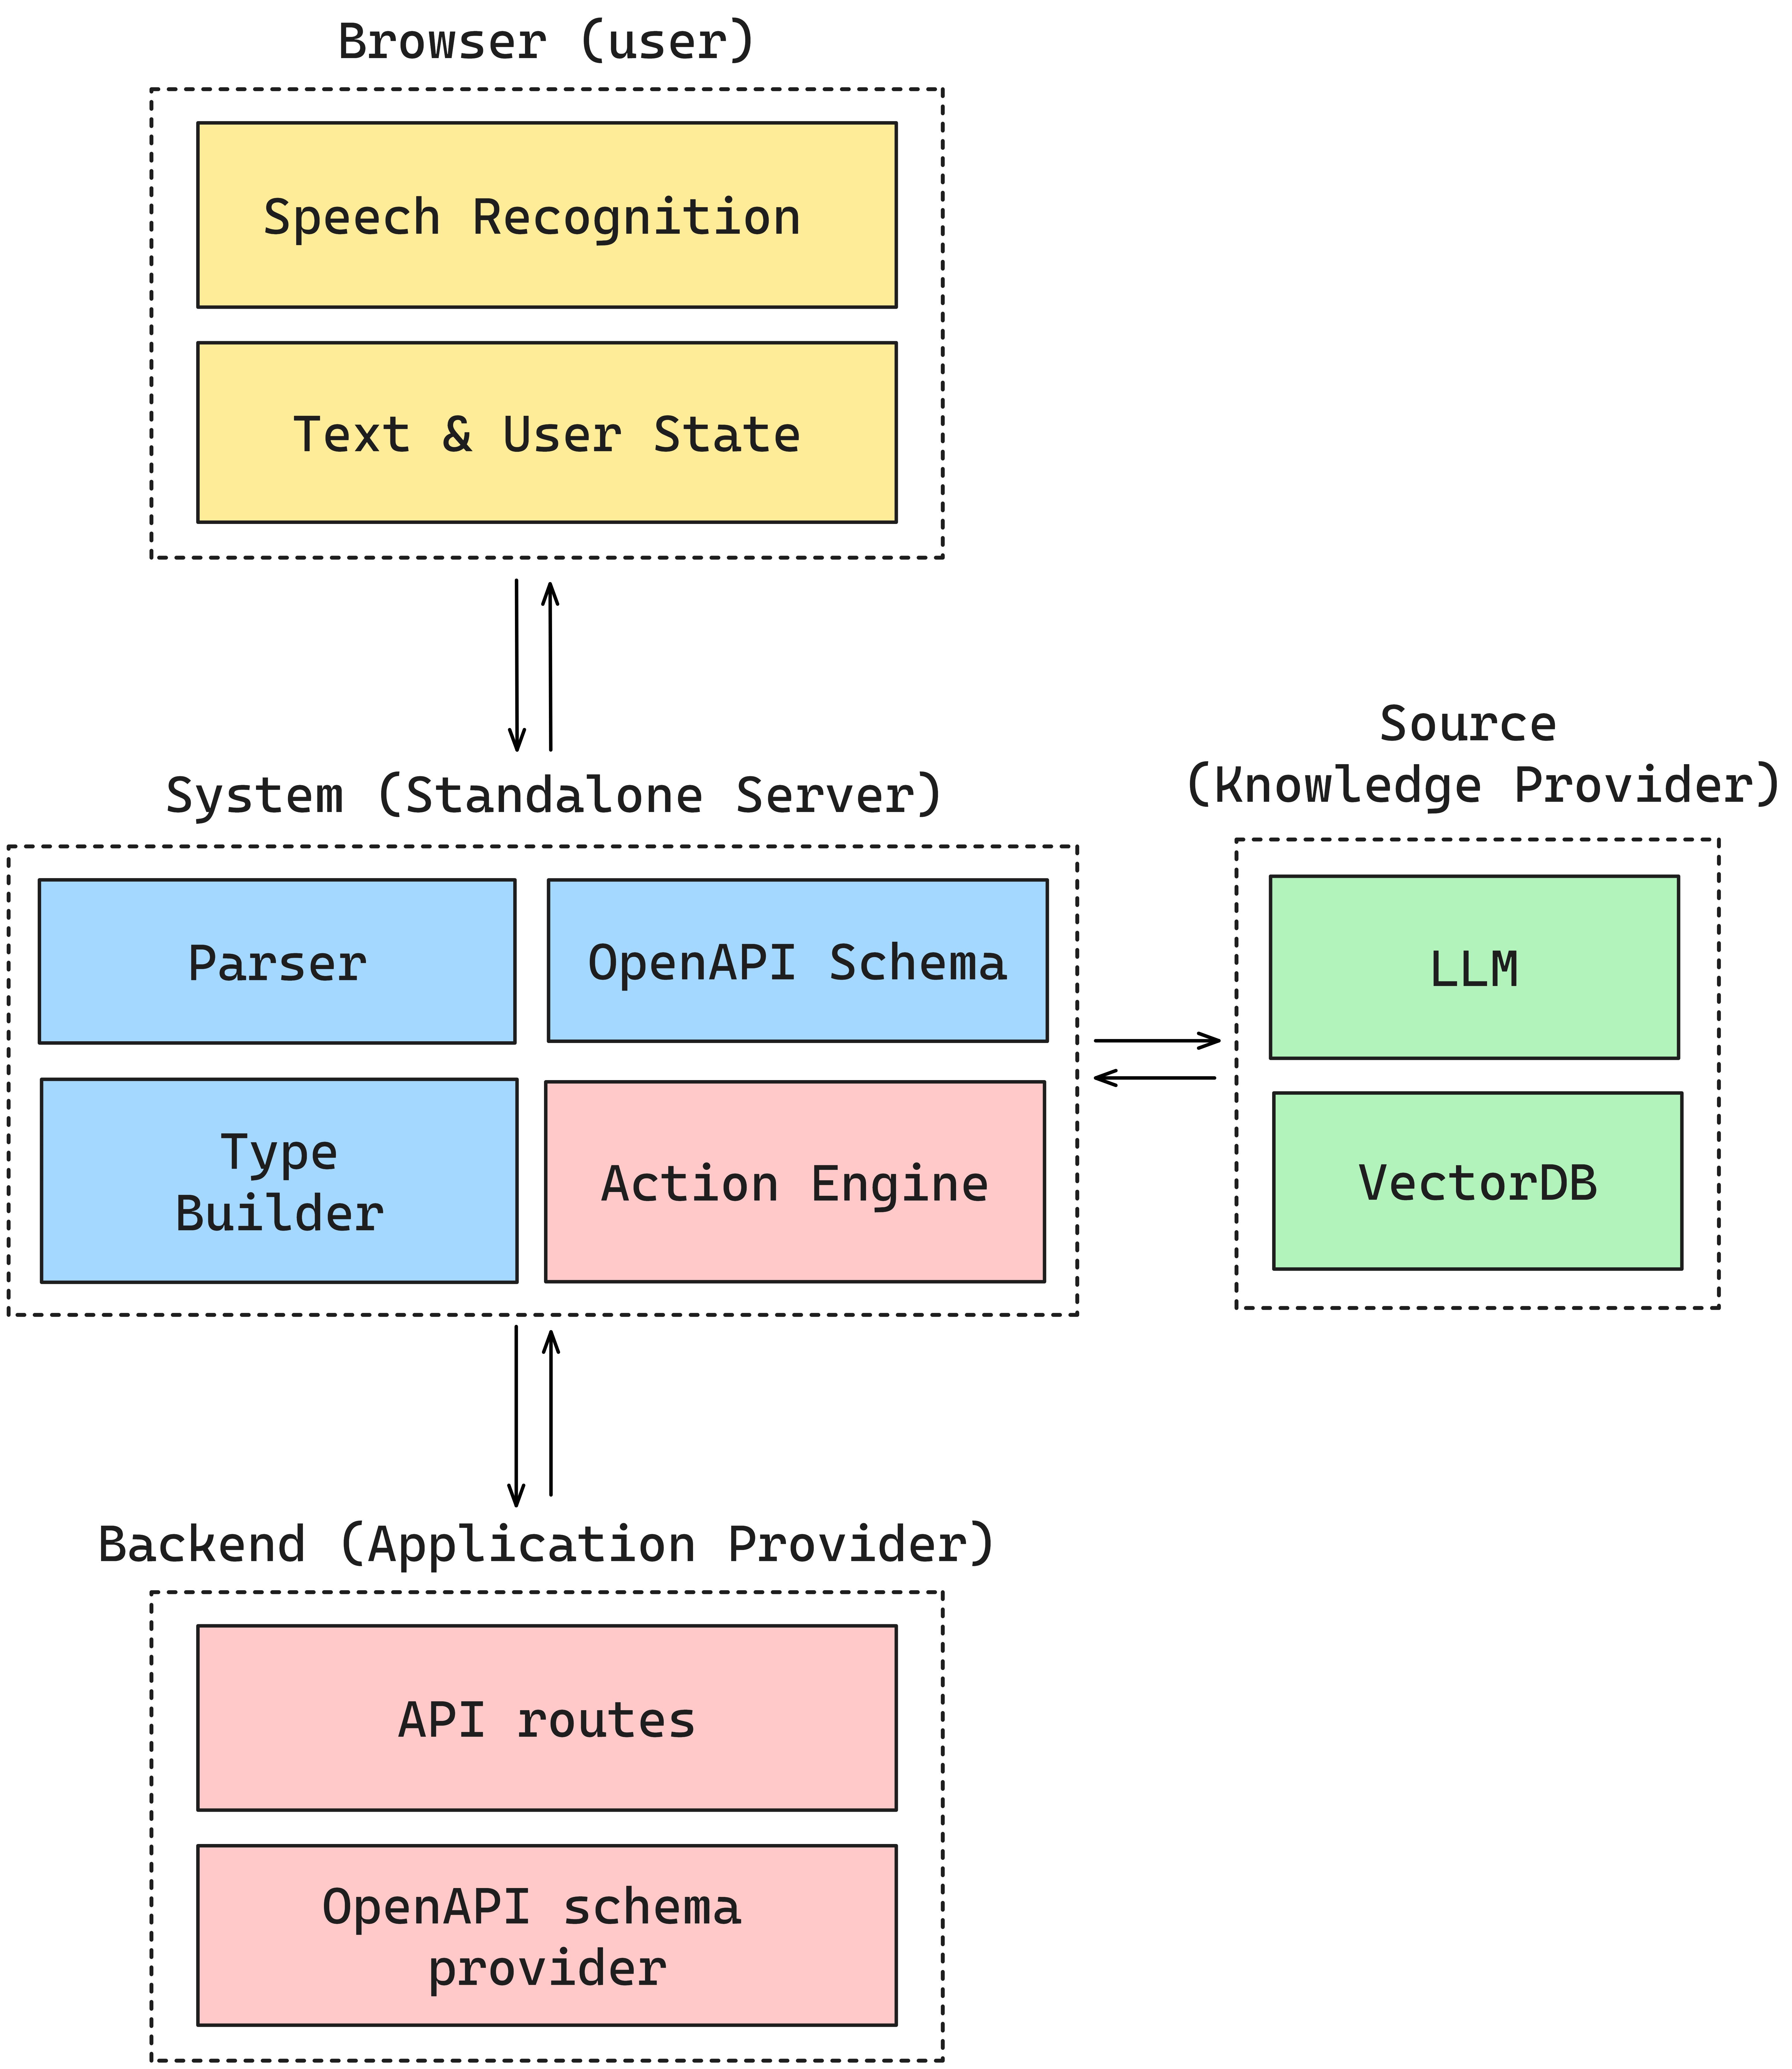
\includegraphics[width=0.5\textwidth]{images/server.png}
    \caption{Simplified Maths problem done with Function Calling.}
    \label{fig}
\end{figure}


\subsection{Action Engine Architecture}
The Action engine architecture follow the same pattern as the build time CLI (CLI that converts the OpenAPI schema to type definitions). Action engine is not an AI system. Currently it is a simple JSON parser that can understand the JSON data from LLM. It turns normal Large Language Model to an Simple Action Model, that enables function calling and chaining. 

Let consider a simple application mathematical calculations, the user asked "what is 10 + 2 / 4" and Action engine had access to all type of mathematical functions. So the LLM return instructions in JSON tag and the Action engine will execute the function in the order of the instructions. The result is then sent back to the user. 


\begin{figure}[htbp]
    \centering
    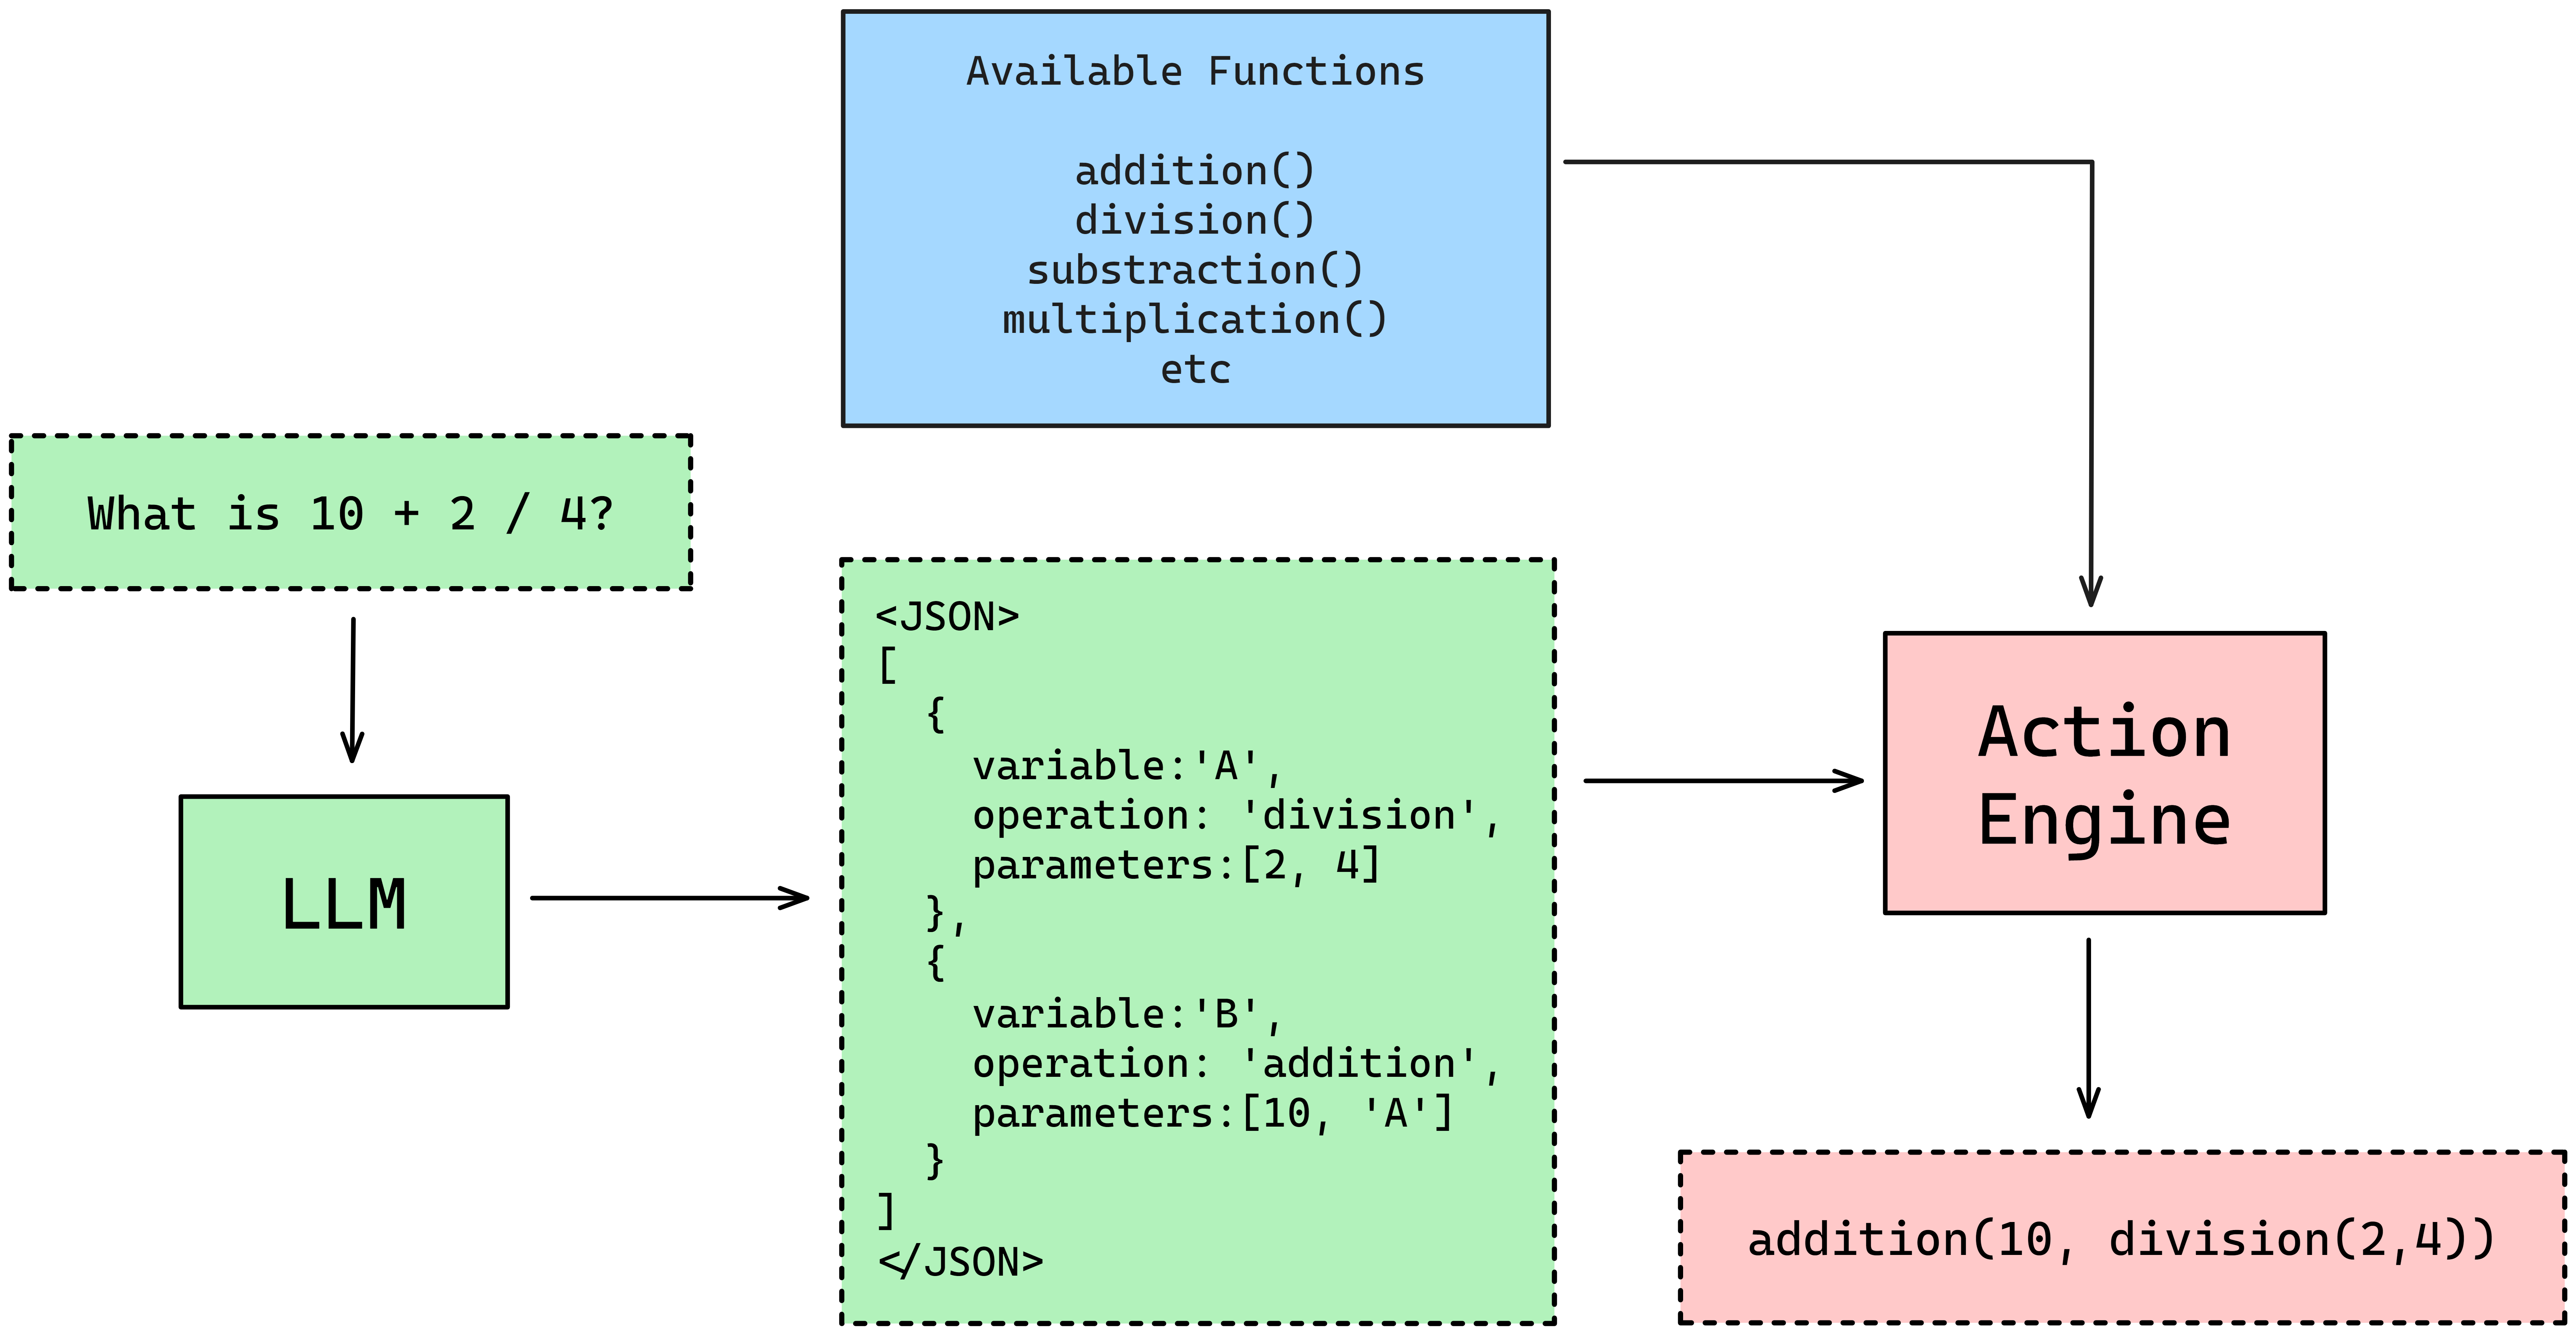
\includegraphics[width=0.5\textwidth]{images/maths.png}
    \caption{Simplified Maths problem done with Function Calling.}
    \label{fig}
\end{figure}

The new unknown variable is generated and used at runtime. Type structure of return JSON can be customized. Here this JSON is enough to represent environment. JSON is parsed and validated by engine and array to moved to execution stack and each function is called sequentially, where result of previous execution is stored in heap at runtime.

\begin{figure}[htbp]
\centering
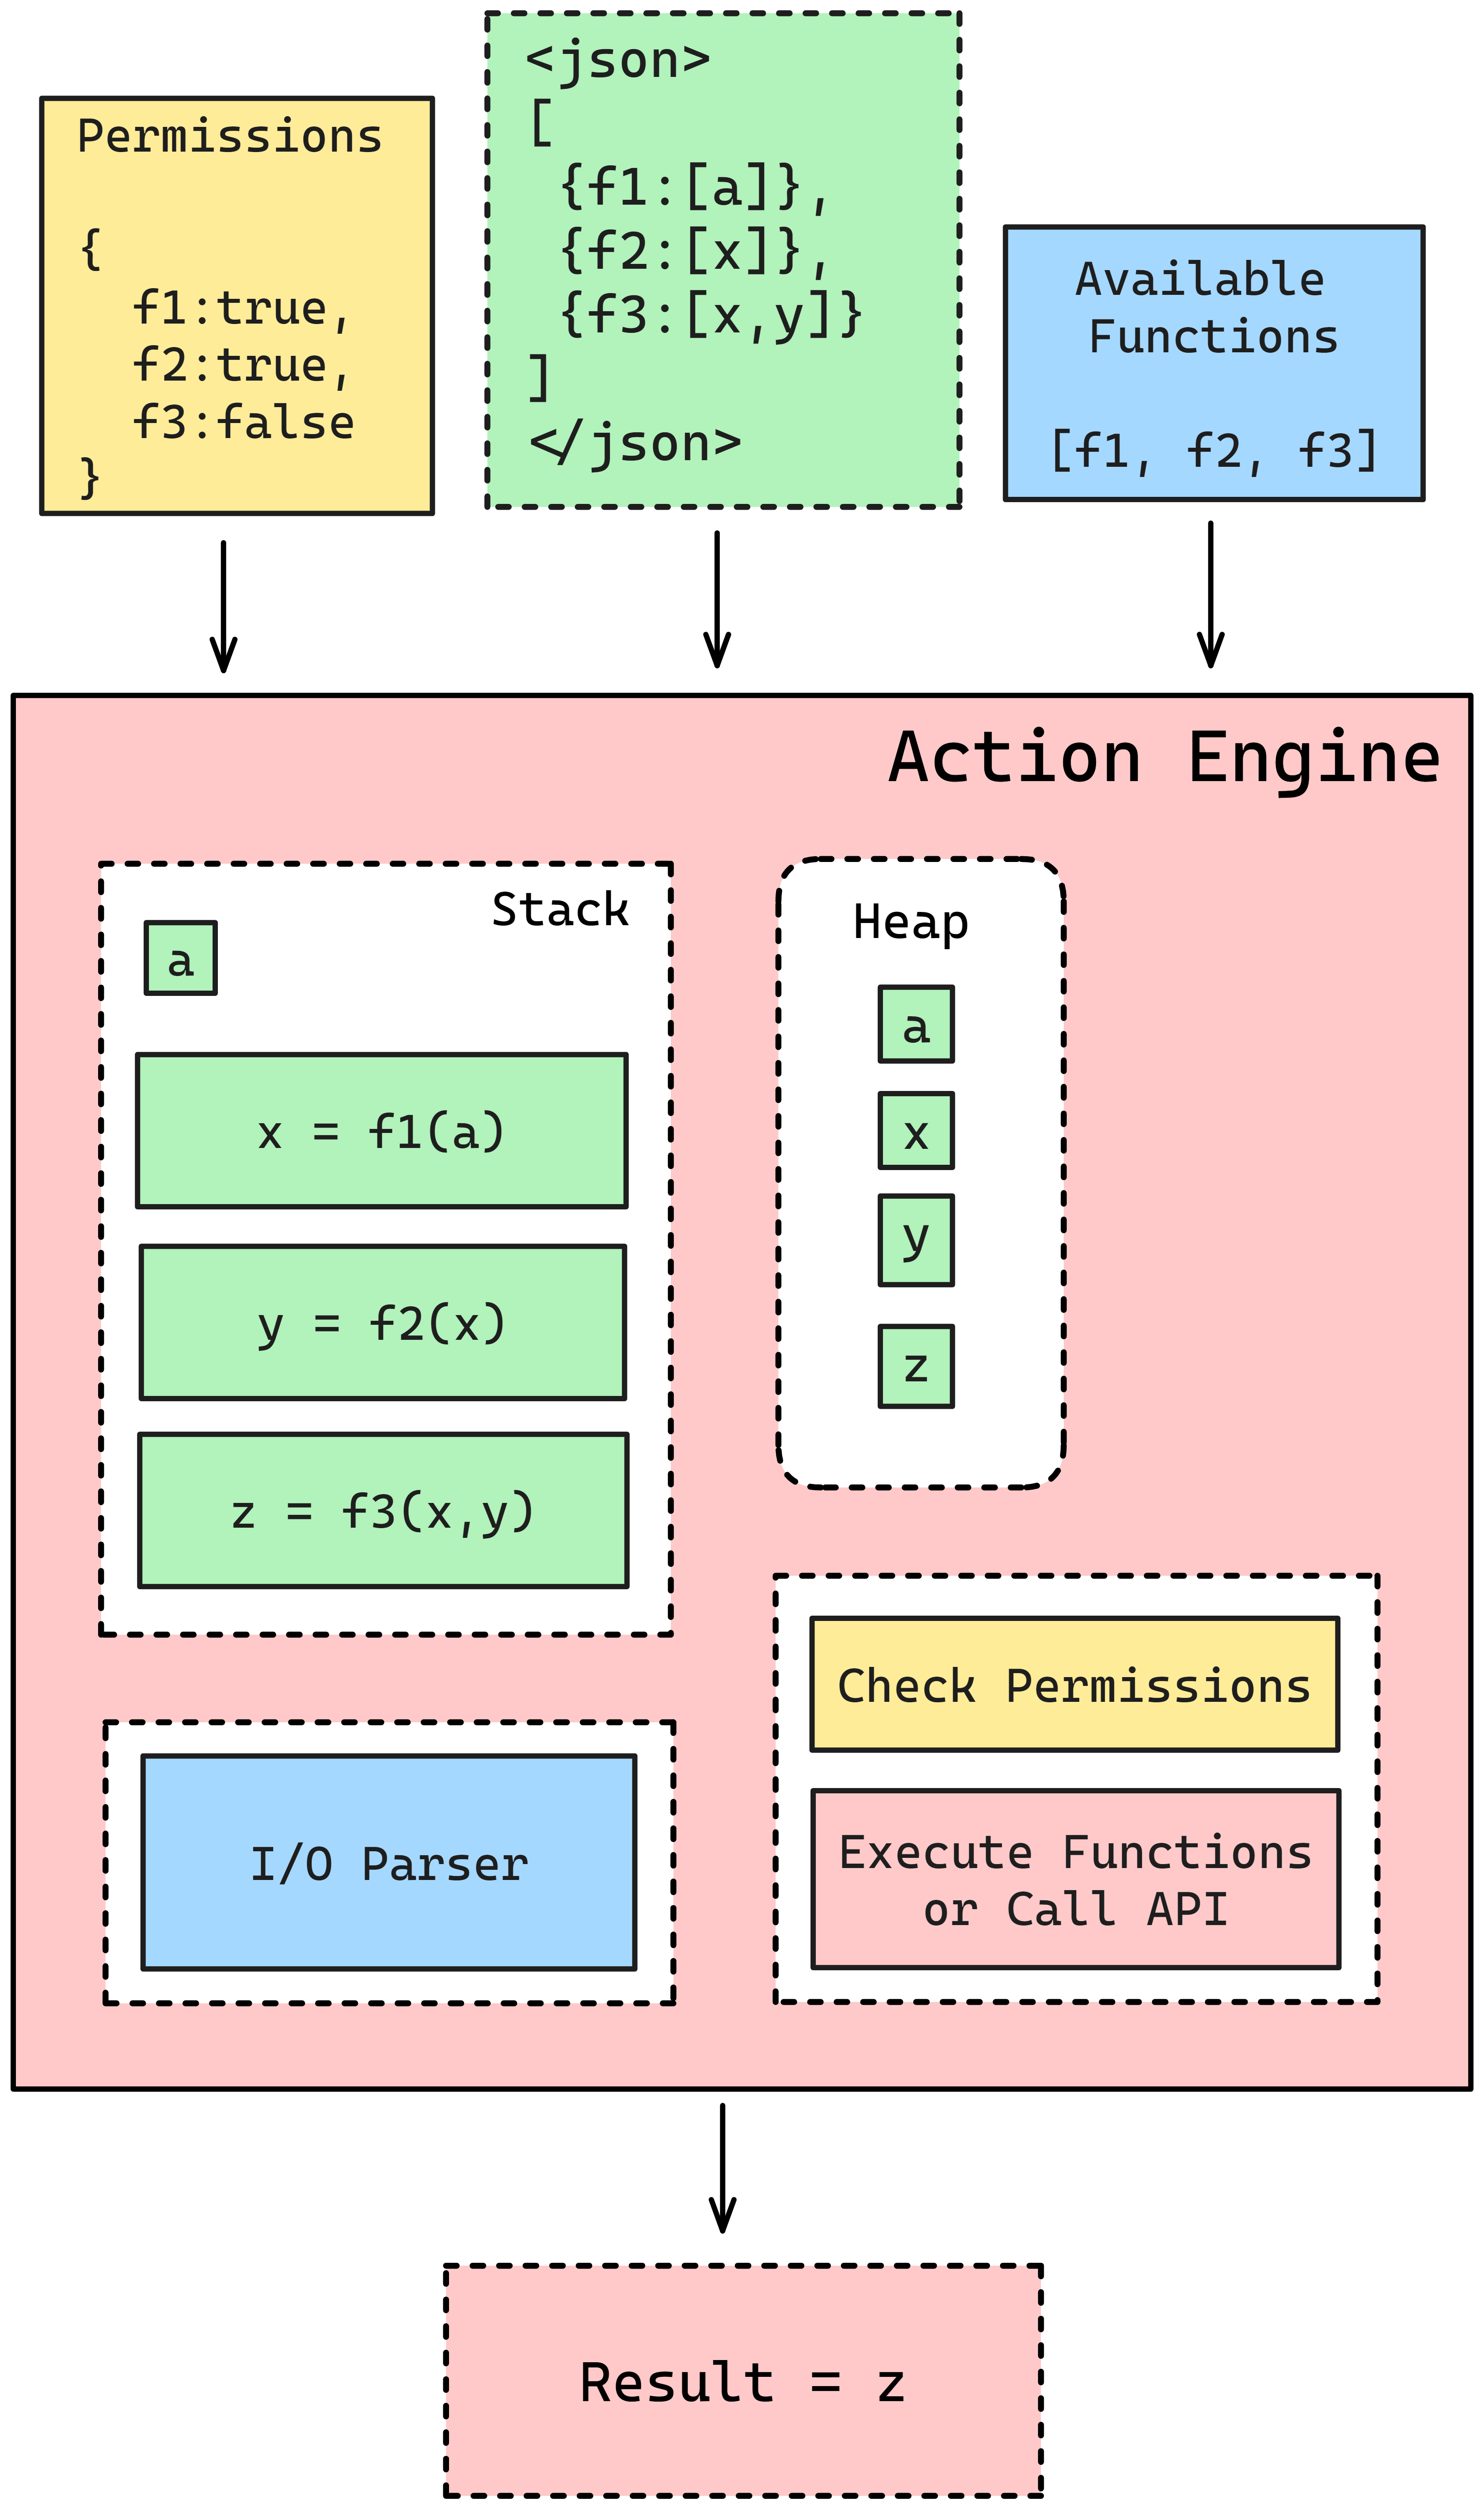
\includegraphics[width=0.5\textwidth]{images/action-engine.png}
\caption{Block Diagram of Action Engine Architecture}
\label{fig}
\end{figure}

Two type of instructions can be evaluated. Single: parse the json, execute the function, done. But for multiple sequential instructions require careful validations and parsing. First execution of function requires complete set of parameters. Always store the executed data and function parameters in heap. If other instructions requires data from previous execution, search in input params list in stack or search heap. If data is not found, return error (and let the server handle that part).

To ensure consistency and compatibility, the input data params and output result from each execution is also validated before passing down to next instructions. This standardization allows for seamless processing and execution of function calling, enabling the system to effectively detect any instances of error made by language model.

The permission is the list of functions that are allowed to run without users concerns. If a function is true, then execute it without asking for permission. If not then return the current result stack of execution back to user and wait until user permits. This feature is crucial while building high secure and user data depended applications. Users don't want any LLM to take decisions and execute some functionalities by its own without their permissions.

% \begin{table}[htbp]
% \caption{VGG16 Classifier}
% \label{tab2} % Label for referencing later
% \begin{center}
% \begin{tabular}{|c|c|}
% \hline
% \textbf{VGG16 parameters} & \textbf{parameter values} \\ % Bold headers
% \hline
% Batch size & 32 \\ % Second row
% \hline
% Epochs& 50 \\
% \hline
% Optimizer& adam\\
% \hline
% Class mode& Categorical\\
% \hline
% loss & categorical\_crossentropy \\

% \hline
% %\multicolumn{2}{l}{$^{\text{a}}$Footnote text here.} % Footnote
% \end{tabular}
% \end{center}
% \end{table}





\subsection{Utilizing Vector storage}
Retrieval Augmented Generation (RAG) is a popular technique used alongside with large language models (LLMs) to improve its performance by including external knowledge sources. Mostly here we can utilize it with help of vector databases. 

OpenAPI schema format supports descriptions and examples. These descriptions can be stored in vector database alongside the meta data of each API routes or components. If the application OpenAPI schema is larger than context window capacity of the LLM, then utilization of vector databases can still reduce the no of request to LLMs. Query the vector database with user prompt and get most probable API route or component. Then combine the results with user prompt to get response from LLM. This approach is faster and efficient than querying the LLMs with large amount of OpenAPI schema.

RAG based Action model is much more efficient when it comes to usage of token while querying. Less the no of tokens used, faster the model respond.

\begin{figure}[htbp]
\centering
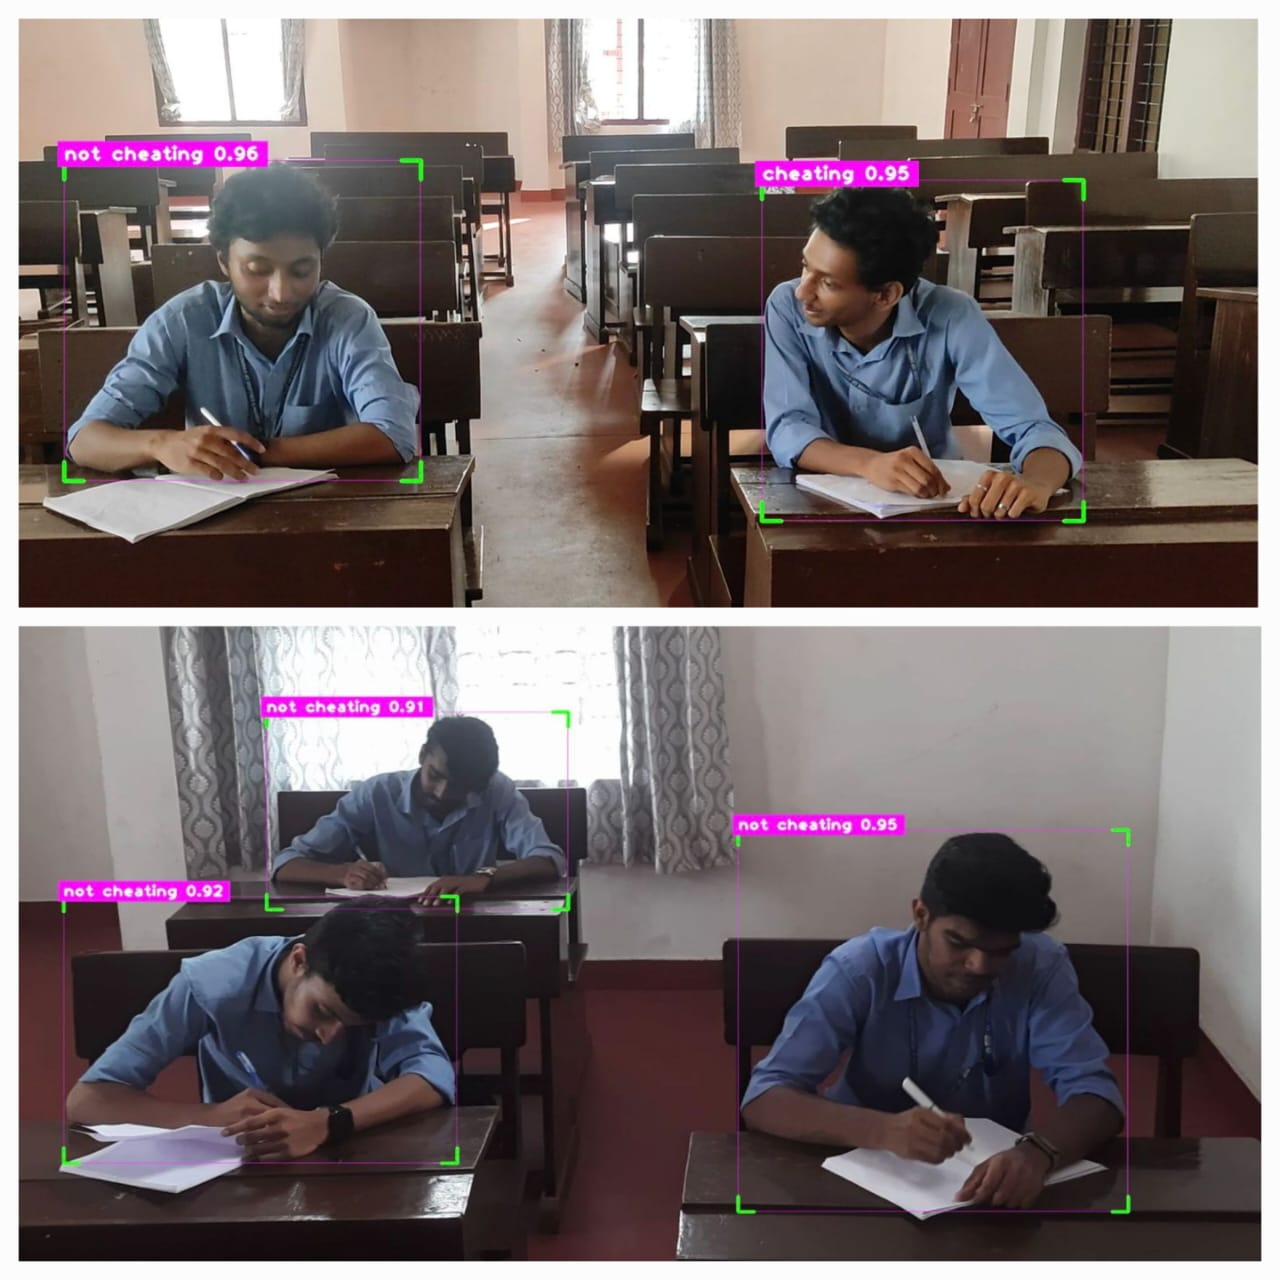
\includegraphics[width=0.5\textwidth, height=10cm]{images/detection.jpeg}  
\caption{Predicted Output From the Model}
\label{fig}
\end{figure}


\subsection{Utilizing runtime validations}
Action models requires strict parsing and validations with OpenAPI schema. LLMs hallucinate sometimes, making it untrust worthy to take decisions. That's why it is important to validate the input and output data from fetching the API. But what if the LLM can just go around the world wide web and fetch the schema of the API and validate at runtime and cache it. This approach is much more futuristic than it sounds. The user prompts, LLM looks for relevant schema from Google search and call those APIs. While system is looking for docs, it can build validators and parsers for the schema at runtime. Also utilize caching mechanism to store the build files for future use. 

It's like google search, but instead of querying, it'll do stuffs online by itself. An inevitable future of language models. 

\subsection{Utilizing multiple calls to LLM}
Popular function calling projects like ReAct utilizes multiple call to LLM to make sure to get the best result and response is moving in right directions. This approach is also useful in Action model. If the response from LLM is not clear or not understandable, then a second call to LLM can be reduce the errors.

This paper was focused on "how to sequentially function call with one query to LLM". But multiple calls to LLM can be useful in some cases. If return data of previously executed function may not be clear or not understandable. Or the data can so long that, without intermediate assistance, it may not reach the end goal as user expected.

\section{Implementation and Result}
\subsection{Implementation}
The study used an advanced object identification model called YOLOv8 (You Only Look Once version 8) to achieve real- time and accurate detection of students in the class. YOLOv8 is widely recognized for its remarkable precision and effectiveness in object recognition, rendering it a perfect match for the specific object detection task. The VGG16 classifies the images into required classes.

A centralized system with a good graphical processor act as the central hub of the entire system which houses an object detection model(YOLOv8)and an image classification model(VGG16)

\subsection{Performance Evaluation}
The result in Table II demonstrates that in the study of YOLOv8 for the detecting the students in exam hall, the model showed outstanding performance across key metrics.
YOLOv8 continuously maintained high precision, as seen by its high Mean Average Precision (mAP) , guaranteeing the accuracy of 95\% in detecting students. It minimized false positives with an exceptional precision score of 0.94. With closely no misses, the model’s recall of 0.96 demonstrated its ability to accurately identify all the  students .
All of these findings demonstrate how reliable and accurate YOLOv8 is an appropriate model to detect students in the classroom, which makes it an important tool for offline exam proctoring.YOLOv8 is the most trending and accurate model which has accuracy close to perfect predictions. combining the state-of-the-art YOLOv8 and VGG16 provided the project with a level of perfection that is unmatchable with humans.Humans has blind spots and other limitations but the EX-GUARD does not have such limitations.

The VGG16 classifier which was trained in house using our custom data set showed some of the best result.the trained model could adapt to the varying demands and situations of the examination hall.The VGG16 Provided an accuracy of 92\% in its evaluation phase.

\begin{figure}[htbp]
\centering
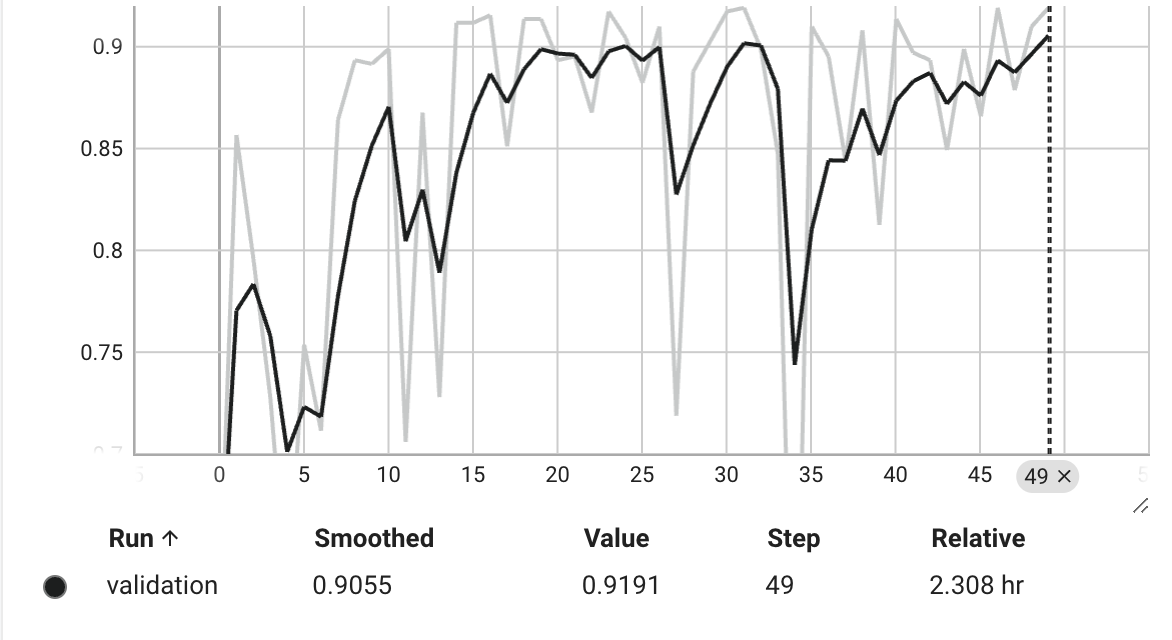
\includegraphics[width=0.5\textwidth, height=7cm]{images/Vgg16acc.png}  
\caption{Accuracy of Vgg16}
\label{fig}
\end{figure}

While comparing with other models like AlexNet, the VGG16 provided better output regarding the ability to classify the student's behaviors. Combining the YOLOv8 and VGG16 the system performed better than the humans. 




\begin{table}[htbp]
\caption{Performance Evaluation:YOLOv8}
\label{tab2} % Label for referencing later
\begin{center}
\begin{tabular}{|c|c|}
\hline
\textbf{Metric} & \textbf{YOLOv8} \\ % Bold headers
\hline
Accuracy & 95\% \\ % Second row

\hline
Precision&0.94\\
\hline
Recall&0.96\\
\hline
 F1-score&0.95 \\

\hline
%\multicolumn{2}{l}{$^{\text{a}}$Footnote text here.} % Footnote
\end{tabular}
\end{center}
\end{table}








\subsection{Findings}
From Fig. 6, which illustrates the usefulness of the YOLOv8
model for detecting students and VGG16 for classification, the study derives a number of noteworthy findings. The following are the main findings:
\begin{enumerate}
    \item  High detection Accuracy: The high Mean Average Precision (mAP) score indicates that the YOLOv8 model typically attained a high level of accuracy. This high accuracy ensures correct detection of exam takers.
    \item High classification accuracy: The high accuracy of VGG16 classifier(92\%) plays a major role in correctly classifying between cheating and non cheating.
     \item Precision and Recall: The model’s 0.94 precision and 0.96 recall scores
highlights its ability to reduce false positives, a crucial
aspect of detecting only students from each frame.
 
    \item Balanced F1-Score: At 0.95, the F1-Score, a measure of
accuracy that is balanced, was observed. This measure
shows that the YOLOv8 model successfully reduces false
positives and false negatives while maintaining good
detection accuracy.
\item Practical Deployment: We have developed a practical and
easily understandable automated proctoring system by integrating pre-trained YOLOv8 model with our custom-trained VGG16 classifier. 


\end{enumerate}


By providing a user-friendly interface for monitoring road
conditions, this system makes real-time analysis and reporting easier.

These indicate the resilience and effectiveness of the YOLOv8
model in detecting students and VGG16 model in classifying the students into "cheating" and "non cheating". The foundation for improved road maintenance and safety is laid by this research,
which may find use in damage prevention and real-time
monitoring.

\subsection{Comparison with State-of-the-Art methods}
In the realm of offline exam proctoring systems, leveraging deep learning models for real-time detection and analysis has become increasingly prevalent. This script integrates several state-of-the-art components, notably utilizing YOLO (You Only Look Once) for object detection, particularly focusing on identifying individuals, typically students, within an exam setting. YOLO offers real-time object detection with impressive accuracy, efficiently bounding boxes around detected objects. YOLOv8 is the best-performing object detection algorithm[17] in the field with the highest accuracy and performance measures.

the system also uses VGG16 classifiers for classifying images, we trained the  AlexNet with the same dataset as that of the VGG16. Referring to Table II, the following outcomes of the comparative study between VGG16 (the proposed model) and AlexNet on the same dataset are shown:
\begin{table}[htbp]
\caption{Comparison of the Performance Metrics for VGG16 and AlexNet}
\label{tab2} % Label for referencing later
\begin{center}
\begin{tabular}{|c|c|c|}
\hline
\textbf{Metric} & \textbf{VGG16} & \textbf{AlexNet} \\ % Bold headers
\hline
Accuracy & 92\% & 64\%\\ % Second row

\hline
Loss&68&76\\
\hline

%\multicolumn{2}{l}{$^{\text{a}}$Footnote text here.} % Footnote
\end{tabular}
\end{center}
\end{table}



\begin{figure}[htbp]
\centering
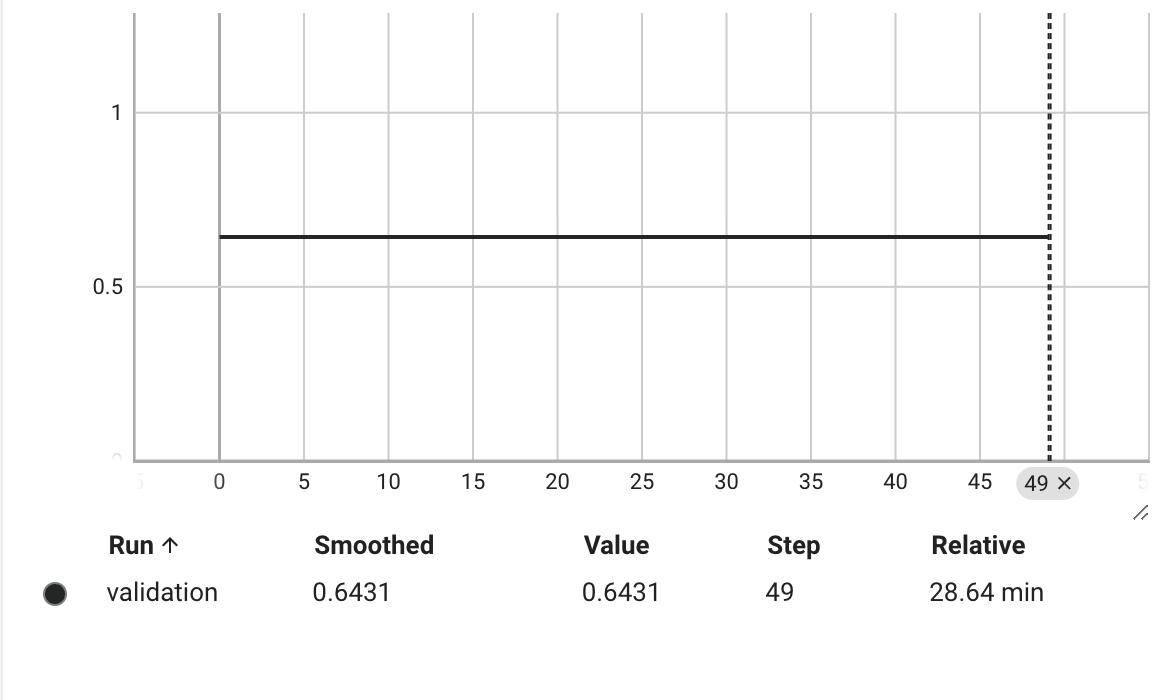
\includegraphics[width=0.5\textwidth, height=7cm]{images/AlexNet.png}  
\caption{Accuracy of AlexNet}
\label{fig}
\end{figure}



\section{Conclusion}
The offline exam proctoring system using AI is an utilization of a combination of YOLO object detection for detecting people in a video stream and a pre-trained VGG16 model for determining whether detected individuals are engaged in cheating behavior during an exam.

In essence, the system processes each frame of the video stream, identifying people using YOLO, and then analyzing each detected person's behavior using the VGG16 model. If the VGG16 model predicts that the person is potentially cheating based on certain features extracted from their behavior or surroundings, such as looking at unauthorized materials, it saves an image of the person for further review. Conversely, if the model determines that the person is not engaged in cheating behavior, it continues processing the video stream. This process is repeated for each frame of the video, allowing the system to continuously monitor and flag potential instances of cheating during an exam.

. 

\section*{References}
[1] Tong Liu ,AI proctoring for offline examinations with 2-Longitudinal-Stream
    Convolutional Neural Networks 10 December 2022
 
[2] Musa Dima Genemo ,Suspicious activity recognition for monitoring cheating in     exams 24 February 2022

[3] Fairouz Hussein , Ayat Al-Ahmad , Subhieh El-Salhi , Esra’a Alshdaifat ,         Mo’taz Al-Hami ,Advances in  Contextual Action Recognition: Automatic 
     Cheating Detection Using Machine Learning Techniques ,31 August 2022

[4] Rhitvik Pasricha ,Prathamesh Churi ,A Systematic Review on AI-based      
    Proctoring Systems: Past, Present  and Future September 2021
    
[5] Joseph Redmon, Santosh Divvala, Ross Girshick, Ali Farhadi You Only   
     Look Once: Unified, Real-Time Object Detection ,9 May 2016

[6] Tanzila Saba, Amjad Rehman, Nor Shahida Jamail1, SouadLarabi Marie-Sainte,
     Mudassar Raza, and Muhammad Sharif Categorizing the Students’ Activities for
     Automated Exam Proctoring using Proposed DeepL2-GraftNet CNN Network and ASO Based Feature Selection Approach, March 2021

[7]  M. Ghizlane, B. Hicham, and F. H. Reda, "A New Modelof Automatic and             Continuous Online Exam Monitoring,"in 2019 International Conference on 
     Systems of Collaboration Big Data, Internet of Things \& Security
    (SysCoBIoTS), 2019, pp. 1-5.

[8]  Mabrouk, A.B., Zagrouba, E.: Abnormal behavior recognition for 
    intel-ligent video surveillance systems: a review. Expert Syst. Appl.
     91,480–491 (2018)

 [9]   He, H., Zheng, Q., Li, R., Dong, B.: Using face recognition to detect
    “Ghost Writer” cheating in examination. In: International Confer-ence on
    E-Learning and Games, pp. 389–397 (2018)

[10] D. Erhan, C. Szegedy, A. Toshev, and D. Anguelov. Scalable
     object detection using deep neural networks. In ComputerVision and Pattern Recognition (CVPR), 2014 IEEE Conference on, pages 2155–2162. IEEE, 2014.

[11] B. Hariharan, P. Arbelaez, R. Girshick, and J. Malik. Simultaneous               detection and segmentation. In Computer Vision–ECCV 2014, pages 297–312.         Springer, 2014.     

[12] Saba, T., Rehman, A., Jamail, N. S. M., Marie-Sainte, S. L., Raza, M.,\&         Sharif, M. (2021).Categorizing the students’ activities for automated exam       proctoring using proposed deep L2-GraftNet CNN network and ASO based             feature selection approach. IEEE Access, 9, 47639–47656. https://doi.org/        10.1109/ACCESS.2021.3068223
[13]Ultralytics Accessed: 04.08.2023 [Online]
    Available: https://www.ultralytics.com/

\end{document}
